\section{Isomap} 

  Isomap is a bit different in the way that it tries to capture more of the global structure of the data, which brings advantages and disadvantages. It is simply a modification of MDS but with geodesic distances. 

  You start off with the point cloud, but with every point, $x_i$, you find the local neighborhood $N_i$ and you make a weighted graph over the whole dataset in the high dimensional space. Then, the distance between any two arbitrary points is the shortest weighted sum of the path between them, calculated by Dijkstra's algorithm. Intuitively, this is an approximation of the geodesic distance, denoted $d_G$, between these two points on a manifold. 
  \begin{figure}[H]
    \centering 
    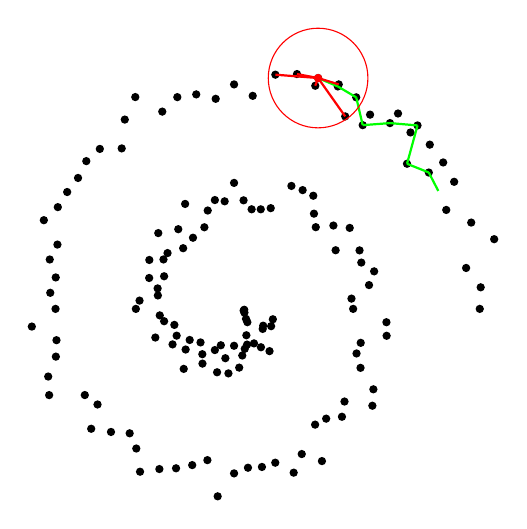
\begin{tikzpicture}
      \pgfmathsetseed{42}
      
      % Store all spiral dot coordinates first
      \foreach \t in {0,5,...,720} {
        \pgfmathsetmacro{\radius}{3 - \t/240}
        \pgfmathsetmacro{\noise}{0.5*rnd}
        \pgfmathsetmacro{\x}{(\radius + \noise) * cos(\t)}
        \pgfmathsetmacro{\y}{(\radius + \noise) * sin(\t)}
        
        \ifnum\t<720
          % Store coordinates globally
          \global\expandafter\edef\csname spiralx\t\endcsname{\x}
          \global\expandafter\edef\csname spiraly\t\endcsname{\y}
          \fill (\x, \y) circle (1.5pt);
        \fi
      }
      
      % Connect a subset of points with green lines (roughly in the top area)
      \pgfmathsetseed{42} % Reset seed to get same coordinates
      \coordinate (prev) at (0,0);
      
      \foreach \t in {30,35,40,45,50,55,60,65,70} {
        \pgfmathsetmacro{\radius}{3 - \t/240}
        \pgfmathsetmacro{\noise}{0.5*rnd}
        \pgfmathsetmacro{\x}{(\radius + \noise) * cos(\t)}
        \pgfmathsetmacro{\y}{(\radius + \noise) * sin(\t)}
        
        % Draw line from previous point (except for first point)
        \ifnum\t>30
          \fill (\x, \y) circle (1.5pt);
          \draw[green, thick] (prev) -- (\x, \y);
        \fi 
        \ifnum\t=70
          \fill[red] (\x, \y) circle (1.5pt);
          \draw[red] (\x, \y) circle (18pt);
          
          % Store red point coordinates
          \pgfmathsetmacro{\redx}{\x}
          \pgfmathsetmacro{\redy}{\y}
          \global\let\redpointx\redx
          \global\let\redpointy\redy
        \fi
        
        % Update previous coordinate
        \coordinate (prev) at (\x, \y);
      }
      
      % Draw red lines from red point to all spiral points within the circle
      \foreach \t in {0,5,...,715} {
        \pgfmathsetmacro{\px}{\csname spiralx\t\endcsname}
        \pgfmathsetmacro{\py}{\csname spiraly\t\endcsname}
        
        % Calculate distance from red point
        \pgfmathsetmacro{\dist}{sqrt((\px - \redpointx)^2 + (\py - \redpointy)^2)}
        
        % If distance is less than circle radius (18pt ≈ 0.25 inches)
        \pgfmathparse{\dist < 0.75 ? 1 : 0}
        \ifnum\pgfmathresult=1
          \draw[red, thick] (\redpointx, \redpointy) -- (\px, \py);
        \fi
      }
    \end{tikzpicture}
    \caption{The classical example is the spiral manifold. The data lies in this manifold, and the geodesic distance helps us gain an accurate distance metric within this data. } 
    \label{fig:isomap}
  \end{figure}

  \begin{definition}[Isomap] 
    Then, we simply do Isomap by minimizing 
    \begin{equation}
      \min_{T} \sum_{i \neq j} \big( d_{\mathbb{R}^k}(T(x_i), T(x_j)) - d_G(x_i, x_j) \big)
    \end{equation}
  \end{definition}

  The problem with this is that it is very sensitive to noise. For example, if we had a few points lying between the spirals, then the geodesic distance between the two spirals would be very small, and so the MDS would try to bring them closer together.  

  \begin{figure}[H]
    \centering
    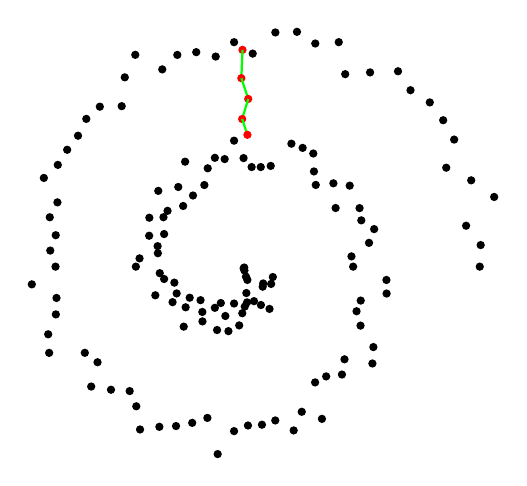
\begin{tikzpicture}
      \pgfmathsetseed{42}
      
      % Draw all spiral dots first
      \foreach \t in {0,5,...,720} {
        \pgfmathsetmacro{\radius}{3 - \t/240}
        \pgfmathsetmacro{\noise}{0.5*rnd}
        \pgfmathsetmacro{\x}{(\radius + \noise) * cos(\t)}
        \pgfmathsetmacro{\y}{(\radius + \noise) * sin(\t)}
        
        \ifnum\t<720
          \fill (\x, \y) circle (1.5pt);
        \fi
      }
      
      % Add red labeled points from top of outermost to second outermost spiral
      % Top of outermost spiral (around 90 degrees, t=90)
      \pgfmathsetseed{42}
      \foreach \step in {1,...,90} {
        \pgfmathsetmacro{\noise}{0.5*rnd}
      }
      \pgfmathsetmacro{\radiusone}{3 - 90/240}
      \pgfmathsetmacro{\noiseone}{0.5*rnd}
      \pgfmathsetmacro{\xone}{(\radiusone) * cos(90)}
      \pgfmathsetmacro{\yone}{(\radiusone) * sin(90)}
      
      % Top of second outermost spiral (around 450 degrees, t=450)
      \pgfmathsetseed{42}
      \foreach \step in {1,...,90} {
        \pgfmathsetmacro{\noise}{0.5*rnd}
      }
      \pgfmathsetmacro{\radiustwo}{3 - 450/240}
      \pgfmathsetmacro{\noisetwo}{0.5*rnd}
      \pgfmathsetmacro{\xtwo}{(\radiustwo + \noisetwo) * cos(90)}
      \pgfmathsetmacro{\ytwo}{(\radiustwo + \noisetwo) * sin(90)}
      
      % Create 7 points total (A, 5 intermediate points, B) with linear interpolation and noise
      \coordinate (prev) at (0,0);
      \foreach \i in {0,1,2,3,4} {
        \pgfmathsetmacro{\t}{\i/4}  % Parameter from 0 to 1
        \pgfmathsetmacro{\interpx}{(1-\t)*\xone + \t*\xtwo}
        \pgfmathsetmacro{\interpy}{(1-\t)*\yone + \t*\ytwo}
        
        % Add some noise to intermediate points
        \pgfmathsetmacro{\noisex}{0.2*rnd}
        \pgfmathsetmacro{\noisey}{0.2*rnd}
        \pgfmathsetmacro{\finalx}{\interpx + \noisex}
        \pgfmathsetmacro{\finaly}{\interpy + \noisey}
        
        % Draw green line from previous point (except for first point)
        \ifnum\i>0
          \draw[green, thick] (prev) -- (\finalx, \finaly);
        \fi
        
        % Draw red point
        \fill[red] (\finalx, \finaly) circle (1.5pt);
        
        % Update previous coordinate
        \coordinate (prev) at (\finalx, \finaly);
      }
    \end{tikzpicture}
    \caption{With extra noisy points (red), the geodesic distance can get corrupted.} 
    \label{fig:isomap_problem}
  \end{figure}

  To fix this, we use \textit{diffusion maps}, which looks at all possible paths between two points and looks at some average of them, which increases robustness. 

